% ===================================================================
% Team 07 - MME / Ichor Systems Universal Plastic Shredder V2.0
% ECE 412/413 Capstone Poster (Spring 2026)
% 48 x 36 in landscape, single page, PSU MCECS look
% ===================================================================
\documentclass[ansiE, landscape]{sciposter}
\usepackage[paperwidth=48in,paperheight=36in,
            left=1.5in,right=1.5in,top=1in,bottom=1in]{geometry}
\setlength{\paperwidth}{48in}
\setlength{\paperheight}{36in}
\setlength{\textwidth}{45in}
\setlength{\textheight}{34in}
\setlength{\oddsidemargin}{0.5in}
\setlength{\evensidemargin}{0.5in}
\setlength{\topmargin}{0in}
\setlength{\headheight}{0pt}
\setlength{\headsep}{0pt}
\setlength{\footskip}{0pt}
\setlength{\columnsep}{0.6in}

\usepackage{multicol}
\usepackage{color}
\usepackage{graphicx}
\usepackage{amsmath}
\usepackage{url}
\usepackage{textcomp}
\usepackage[skins,breakable,raster]{tcolorbox}
\usepackage{tikz}
\usepackage{adjustbox}

% PSU palette
\definecolor{PSUgreen}{RGB}{106,127,16}
\definecolor{PSUltgreen}{RGB}{168,180,0}
\definecolor{PSUblue}{RGB}{0,117,154}
\definecolor{PSUltblue}{RGB}{161,216,224}
\definecolor{PSUgray}{RGB}{71,67,52}
\definecolor{PSUred}{RGB}{210,73,42}
\definecolor{PSUorange}{RGB}{220,155,50}
\definecolor{PSUcream}{RGB}{250,247,238}

% Typography
\renewcommand{\LARGE}{\fontsize{96pt}{106pt}\selectfont}
\renewcommand{\Large}{\fontsize{58pt}{64pt}\selectfont}
\renewcommand{\large}{\fontsize{30pt}{36pt}\selectfont}
\renewcommand{\normalsize}{\fontsize{18pt}{22pt}\selectfont}
\renewcommand{\titlesize}{\LARGE}
\renewcommand{\authorsize}{\Large}
\renewcommand{\instsize}{\large}

% Empty out the default sciposter title -- we draw our own banner
\title{}
\author{}
\institute{}
\conference{}
\renewcommand{\footlogo}{}

% Custom section header: green pill with white text + tiny shadow line under
\newcommand{\postersec}[1]{%
  \par\vspace{6pt}%
  \noindent
  \begin{tcolorbox}[
    enhanced, sharp corners, boxrule=0pt, frame hidden,
    interior style={top color=PSUgreen, bottom color=PSUgreen!90!black},
    coltext=white,
    left=14pt, right=14pt, top=6pt, bottom=6pt,
    width=\linewidth,
    fontupper=\sffamily\bfseries\large,
    drop shadow=PSUgray!40,
  ]
  #1
  \end{tcolorbox}%
  \par\vspace{4pt}
}

% Wide colored cards inside a tcbraster (for the highlights strip)
\newtcolorbox{statcard}[1]{enhanced, sharp corners, boxrule=0pt, frame hidden,
  interior style={top color=PSUcream, bottom color=white},
  borderline north={3pt}{0pt}{PSUgreen},
  left=12pt, right=12pt, top=8pt, bottom=10pt,
  fontupper=\sffamily, title=#1, coltitle=PSUgreen,
  fonttitle=\sffamily\bfseries\large,
  attach title to upper={\par\smallskip}}

\begin{document}

% ============== TITLE BANNER (replaces default \maketitle) ==============
\noindent
\begin{tcolorbox}[
  enhanced, sharp corners, boxrule=0pt, frame hidden,
  interior style={top color=PSUgreen, bottom color=PSUltgreen},
  coltext=white,
  left=30pt, right=30pt, top=18pt, bottom=18pt,
  width=\textwidth,
  fontupper=\sffamily,
]
\begin{minipage}[c]{0.80\linewidth}
  {\fontsize{90pt}{96pt}\selectfont\bfseries
   UNIVERSAL PLASTIC SHREDDER V2.0}\\[6pt]
  {\fontsize{40pt}{46pt}\selectfont\bfseries Electrical Control \& Power System}\\[14pt]
  {\fontsize{28pt}{32pt}\selectfont
   Bao Nguyen\;\textbullet\;Fearghus Tyler\;\textbullet\;Yaqoub Rabiah\;\textbullet\;Fox Kang}\\[6pt]
  {\fontsize{22pt}{26pt}\selectfont
   Portland State University\,\textbullet\,MCECS\,\textbullet\,Department of Electrical \& Computer Engineering}\\[2pt]
  {\fontsize{22pt}{26pt}\selectfont
   Sponsor: MME / Ichor Systems (Bridget Lannigan)\quad\textbar\quad
   Advisors: Prof.~Andrew Greenberg, Dr.~Jonathan Bird (EE), Robert Paxton (ME)}
\end{minipage}\hfill
\begin{minipage}[c]{0.16\linewidth}
  \raggedleft
  
\includegraphics[height=2.6in]{./Logo/psuMCECSloghoriz.png}
\end{minipage}
\end{tcolorbox}

\vspace{12pt}

\begin{multicols}{3}

%================ COLUMN 1 ================
\postersec{The Problem}
Ichor Systems generates large volumes of thick rigid plastic
(PVC, PP, LDPE) during semiconductor equipment manufacturing.
Off-the-shelf shredders are either too small for the material
(0.25--0.5\,in.~sheets, 4--12\,in.~wide) or priced far above the
sponsor's per-line budget. The EE team designed and built the
electrical control and power system for an industrial-grade
plastic shredder; the mechanical structure is delivered by a
separate ME team.

\postersec{Requirements}
\textbf{Must:}
\begin{itemize}\setlength{\itemsep}{2pt}
  \item Shred plastic to $\sim$1\,in.~pieces.
  \item Drive a 3--5\,HP motor at 70--90\,RPM through a controllable VFD.
  \item Follow NFPA 70 (NEC); include E-stop, overload, and one safety interlock.
  \item Provide an HMI for operator control and status.
  \item Stay within the \$1{,}000 EE-team budget.
\end{itemize}
\textbf{Should:} status / fault lights, NEMA enclosure, labeled controls. \\
\textbf{May:} read-only wireless monitoring, data logging, capacitive-touch safety.

\postersec{System Architecture}
The control system is built end-to-end on AutomationDirect industrial
hardware -- no hobby-grade microcontrollers are in the safety or
control path. A PowerTec 71008 disconnect feeds a Mean Well NDR-480-24
24\,VDC supply, a Mitsubishi SD-N35 contactor (E-stop hardwired in
series with its coil), and a Huanyang HY02D211B-T VFD. The VFD drives
a 3\,HP bench motor (GE 5KE182BC205B) over U/V/W via blue, white, and
red 4\,mm banana sockets.

\begin{center}
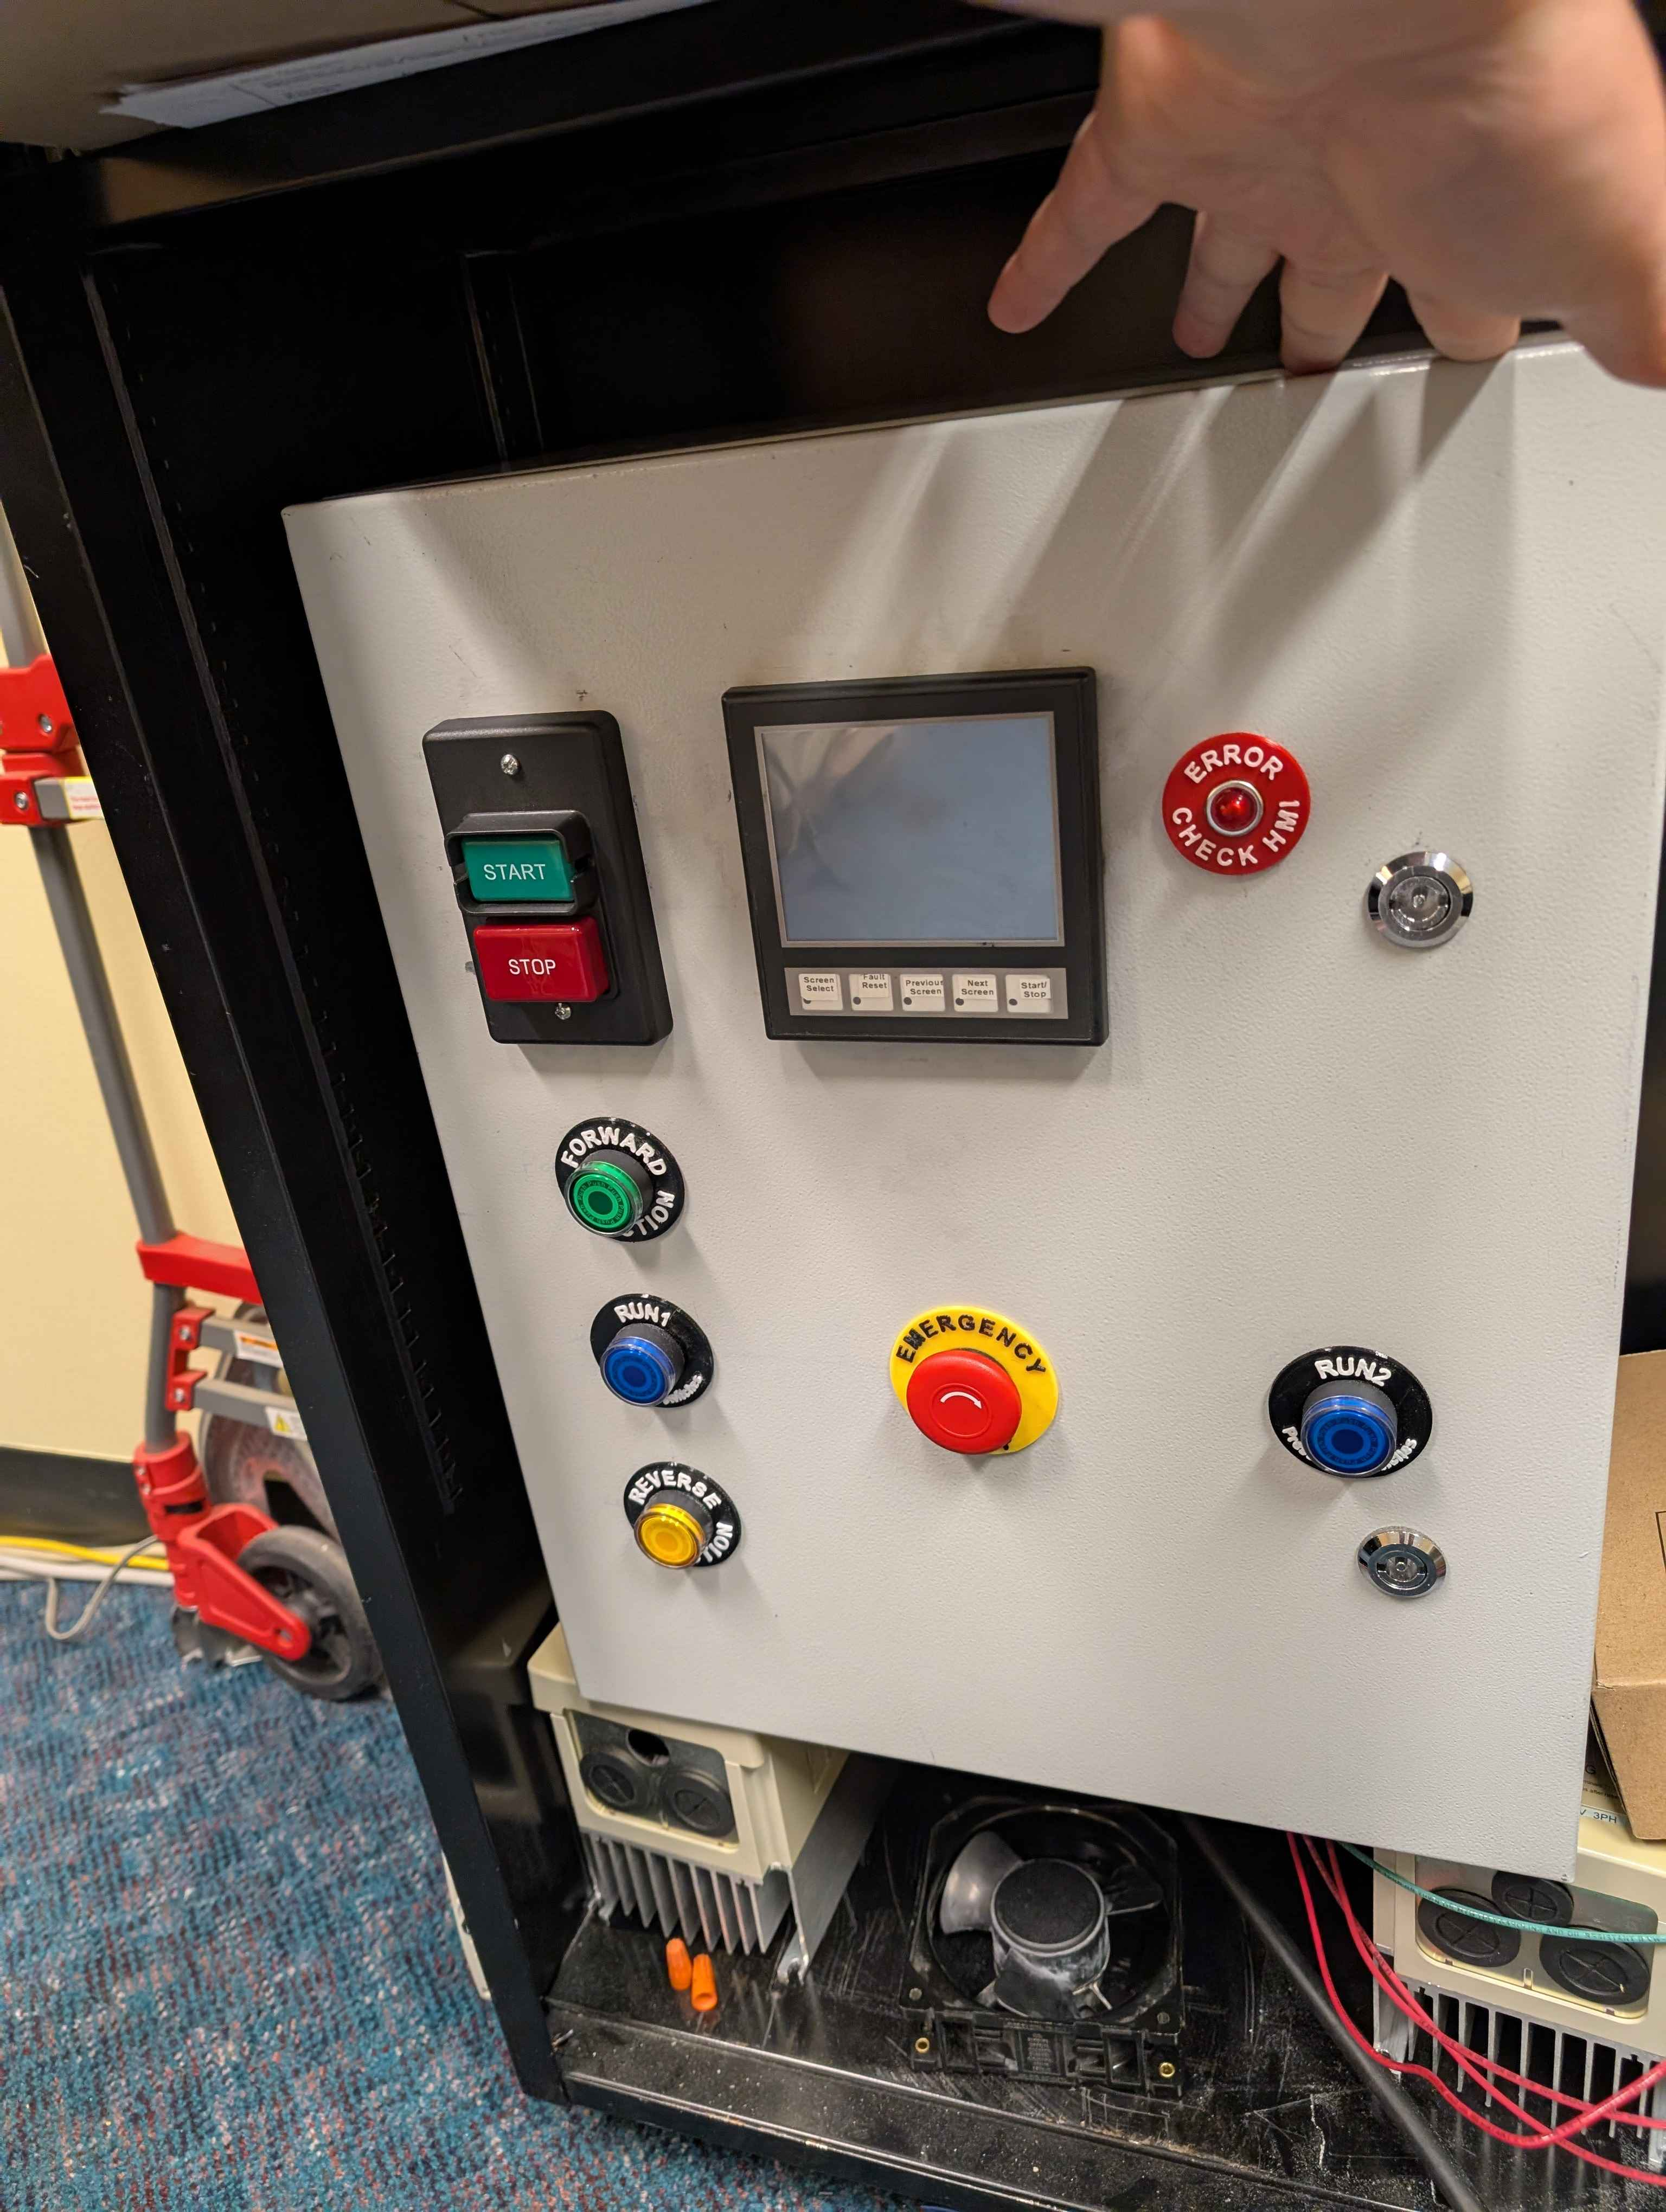
\includegraphics[height=7in]{./Pictures/Photo_Front_Panel.jpg}\hspace{6pt}%
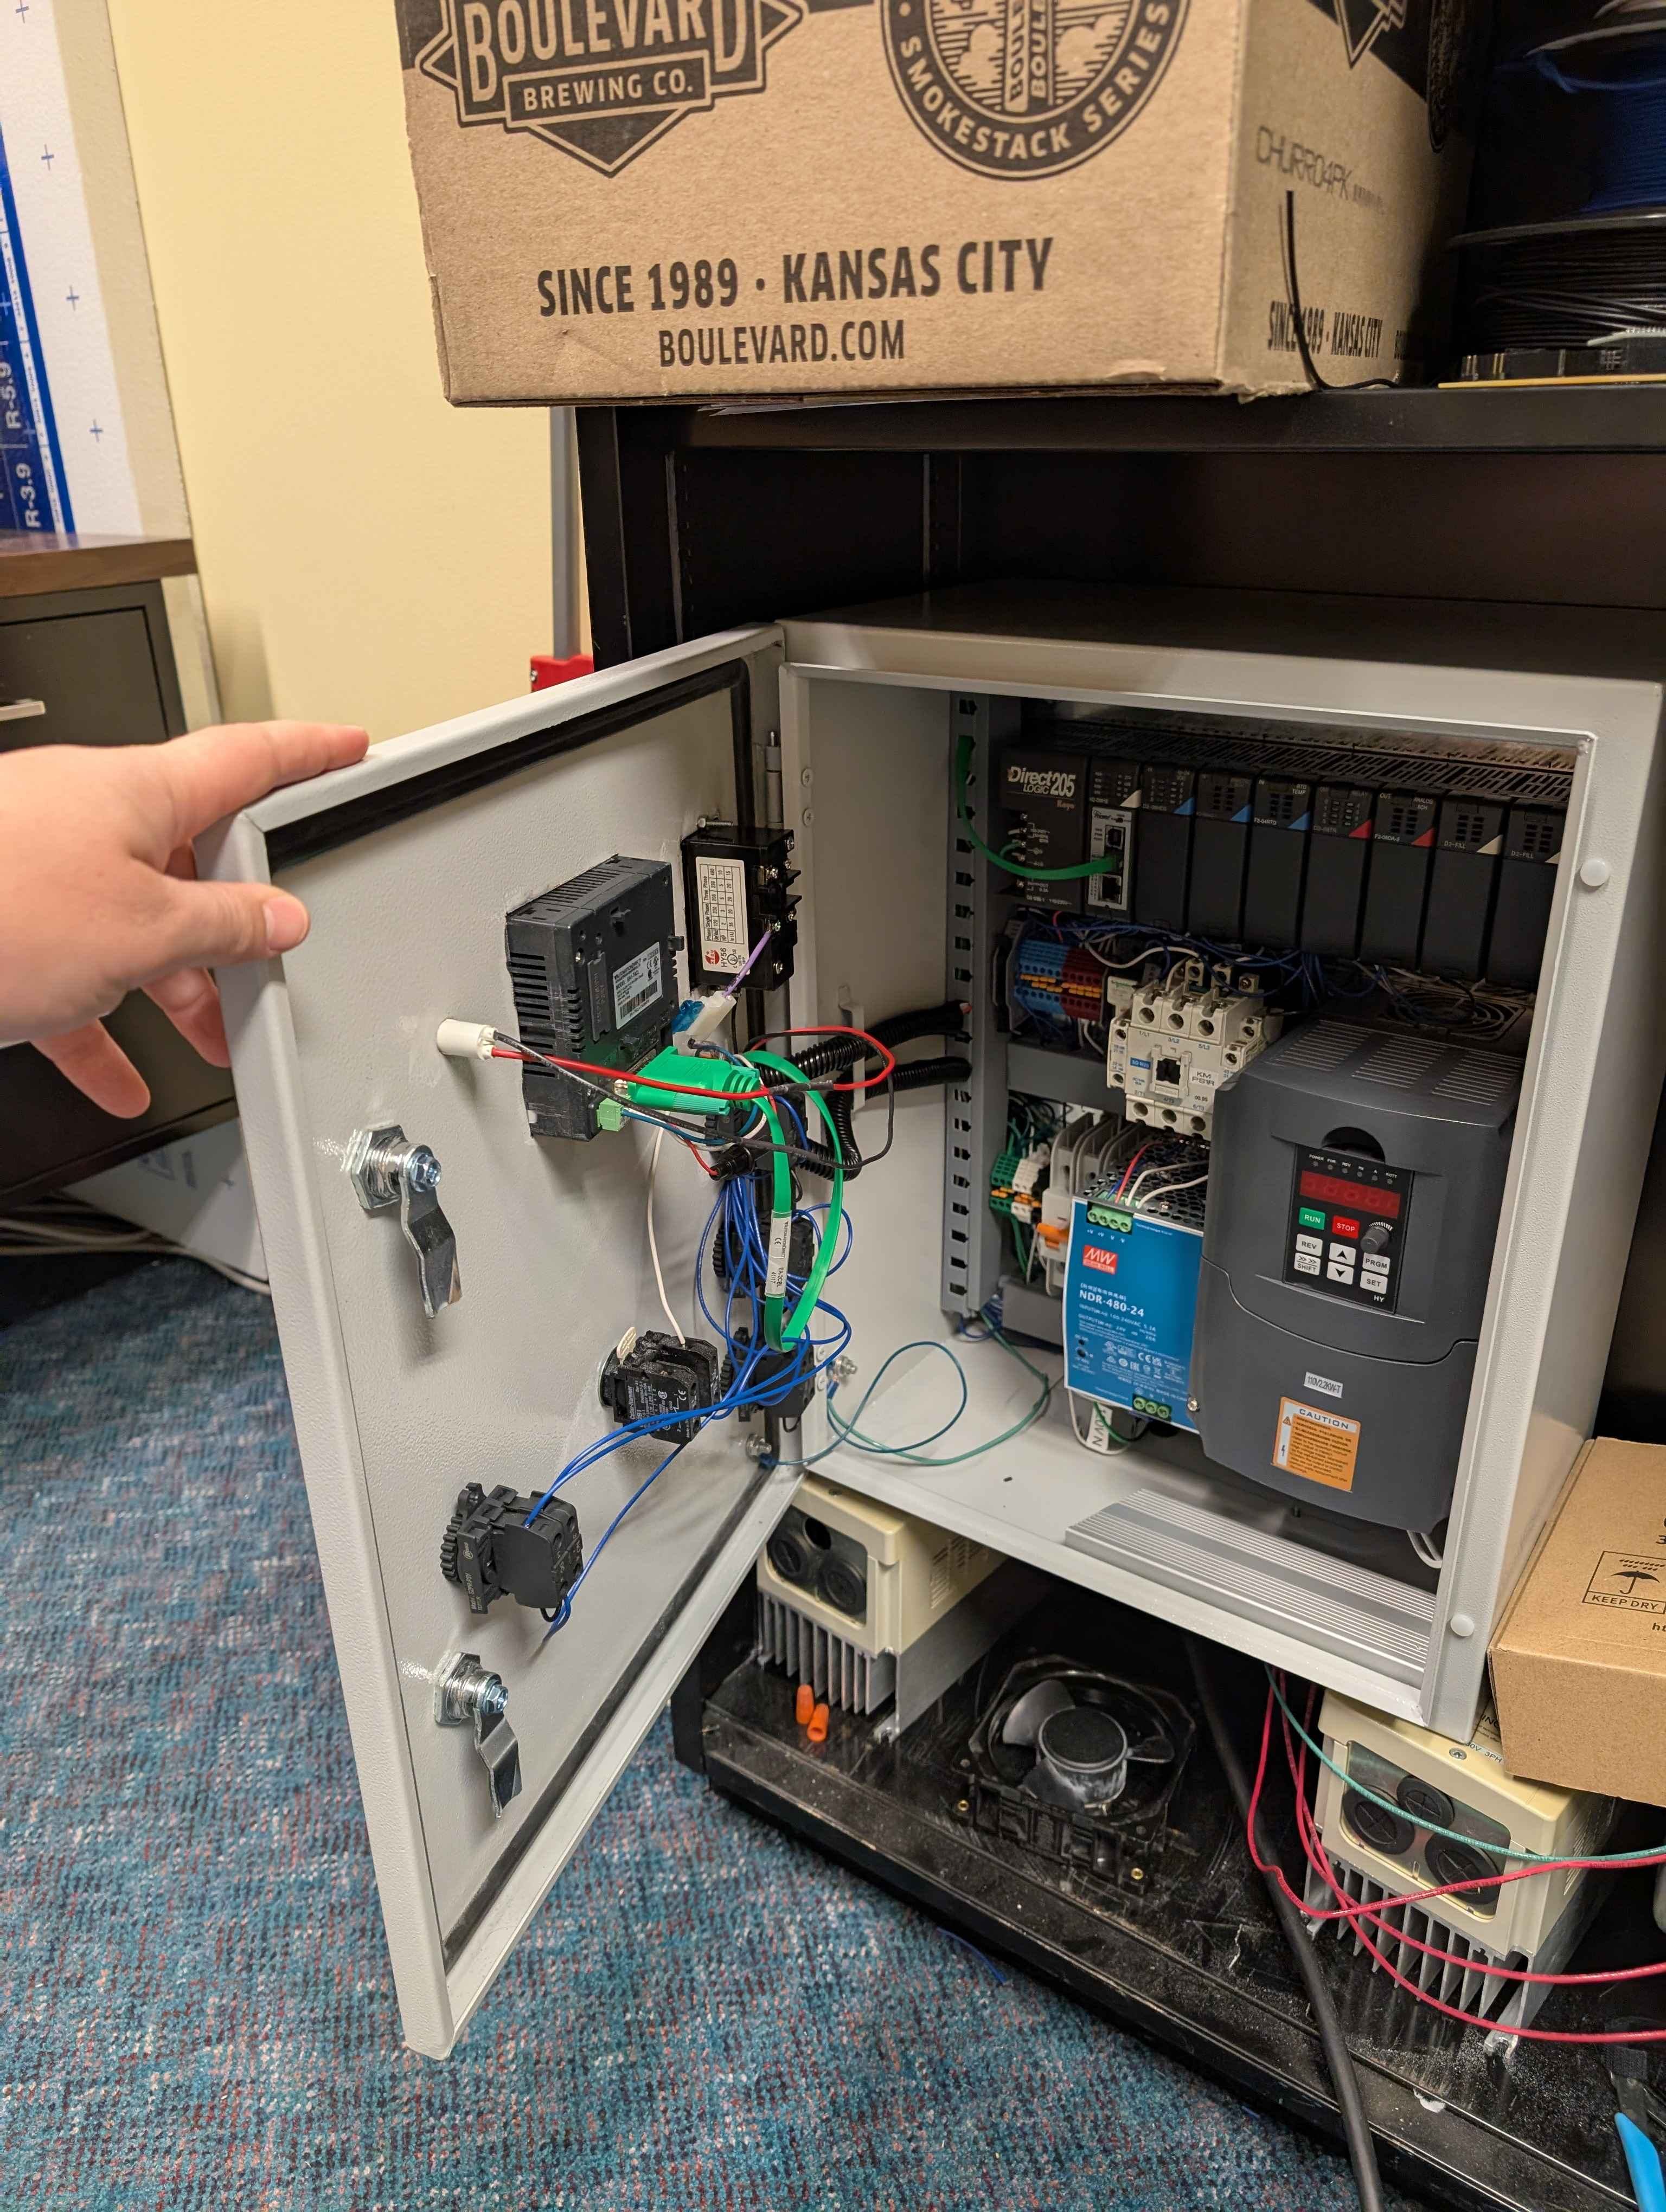
\includegraphics[height=7in]{./Pictures/Photo_Inside_Panel.jpg}\\[3pt]
{\small\itshape As-built operator face (left) and panel interior (right): EA1-T4CL HMI, deadman / forward / reverse / E-stop, DirectLOGIC 205 rack, Huanyang VFD, 24\,VDC supply, SD-N35 contactor, and fused terminal blocks.}
\end{center}

\columnbreak
%================ COLUMN 2 ================
\postersec{PLC Control \& Ladder Logic}
The PLC is the system controller. A DirectLOGIC 205 D2-09B-1 rack
holds the H2-DM1E CPU and five I/O modules: \texttt{D2-08ND3}
(8 DC inputs), \texttt{F2-08AD-1} (analog current input),
\texttt{F2-04RTD} (RTD), \texttt{D2-08TR} (8 relay outputs), and
\texttt{F2-08DA-2} (0--10\,V analog output to the VFD). The 31-rung
Do-more program implements a deterministic state machine plus a
3-strike jam recovery sequence and a hard-lockout path.

\begin{center}
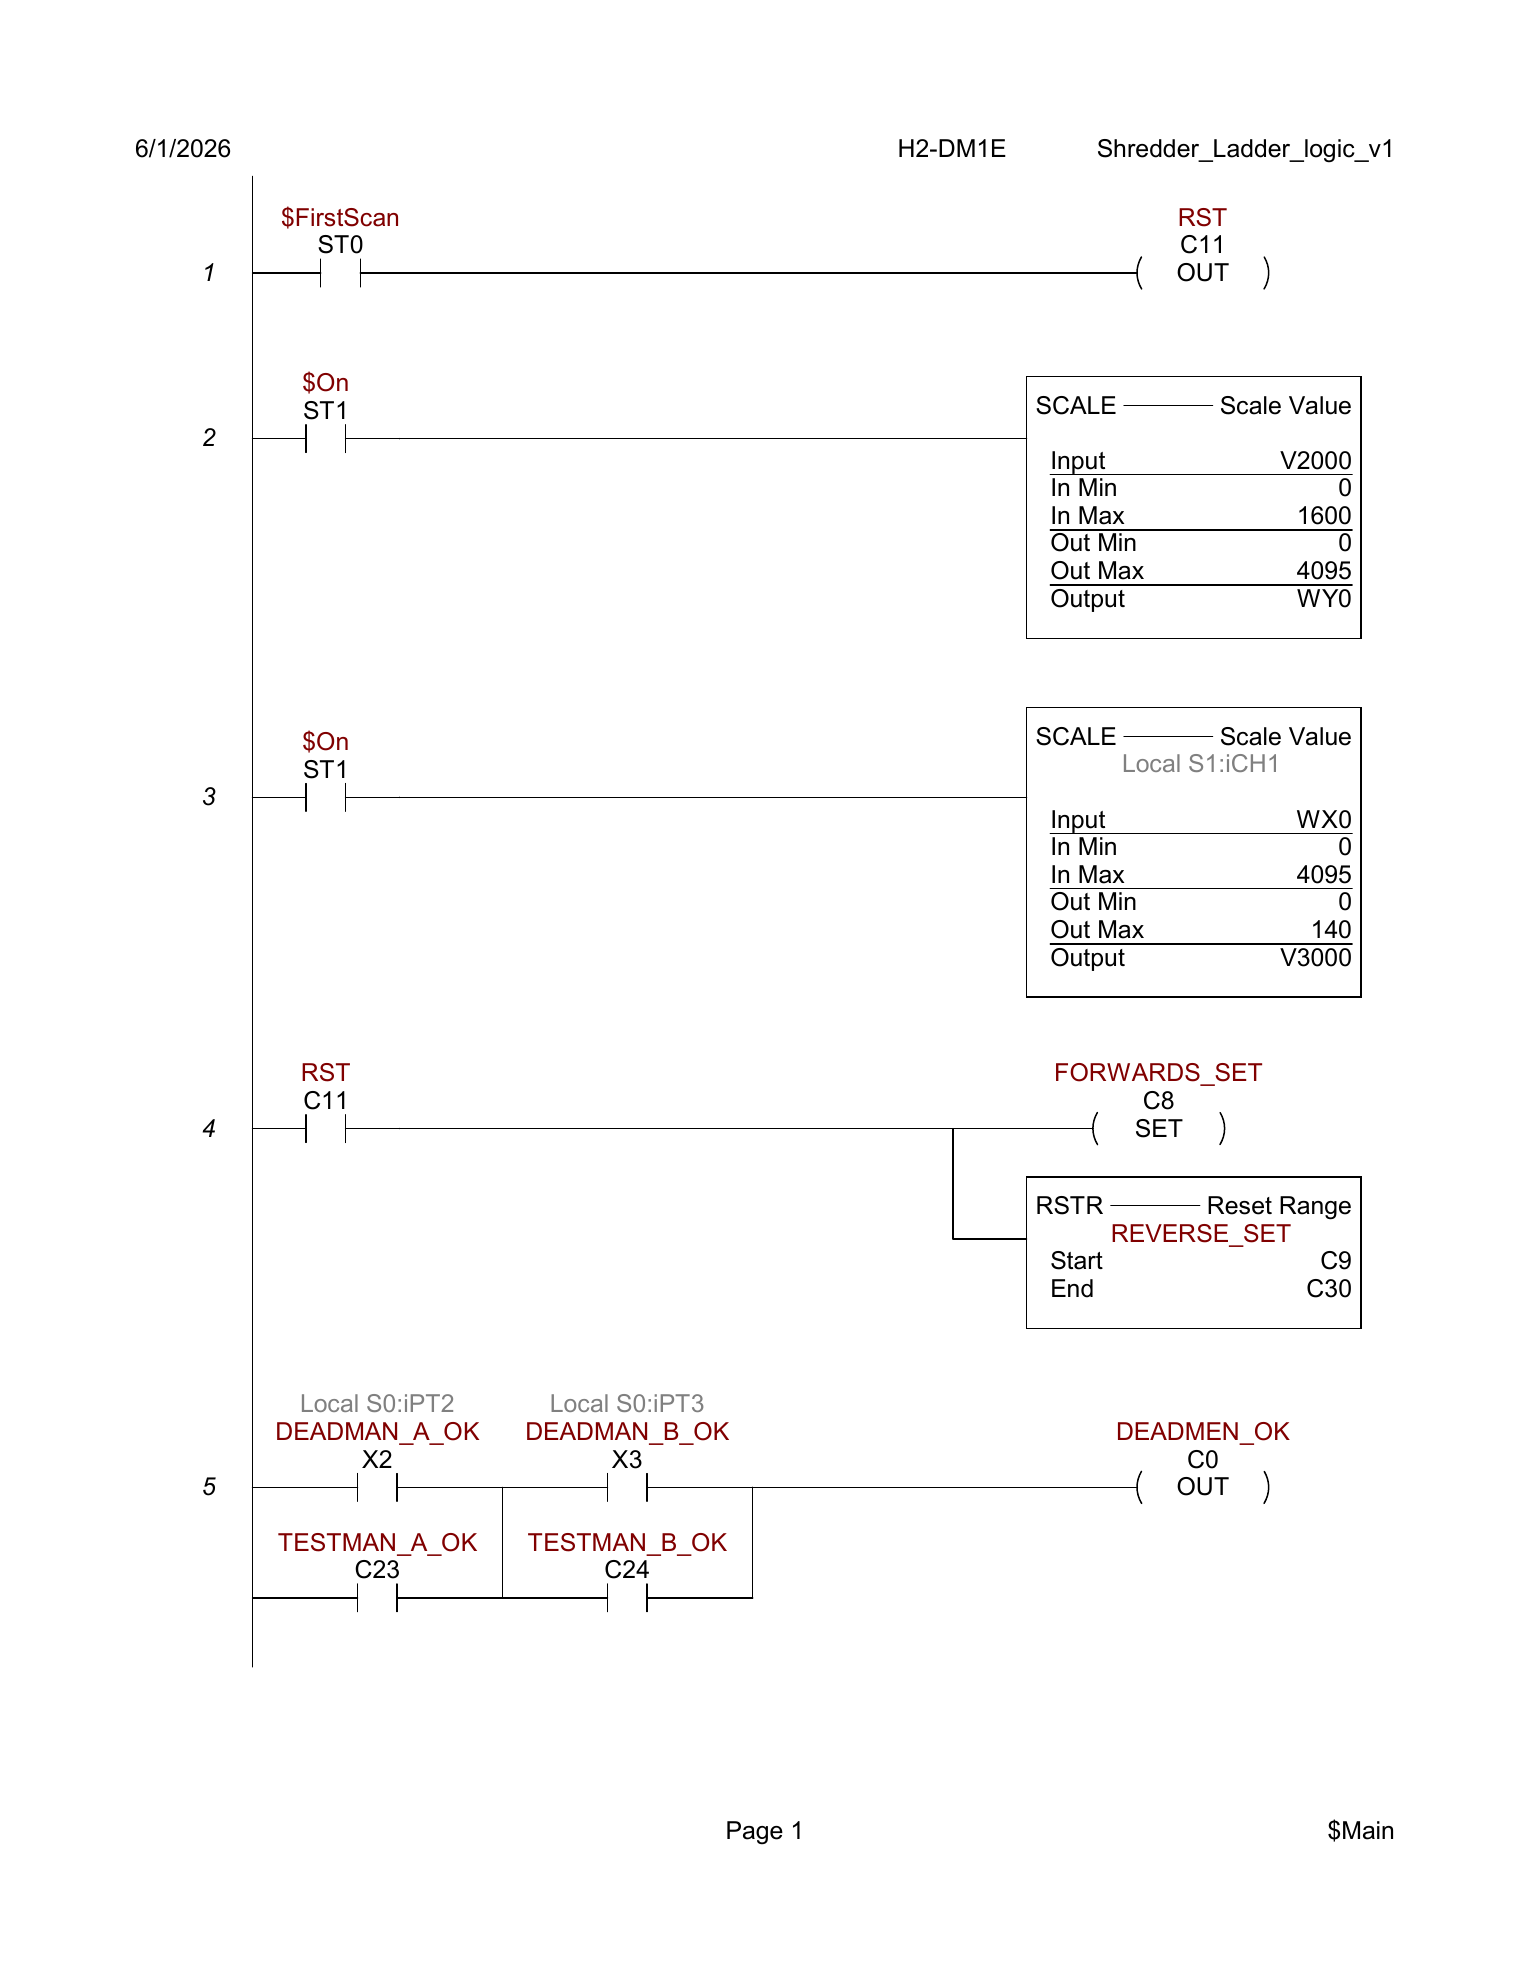
\includegraphics[height=2.1in]{./Pictures/Ladder_1.png}\hspace{6pt}%
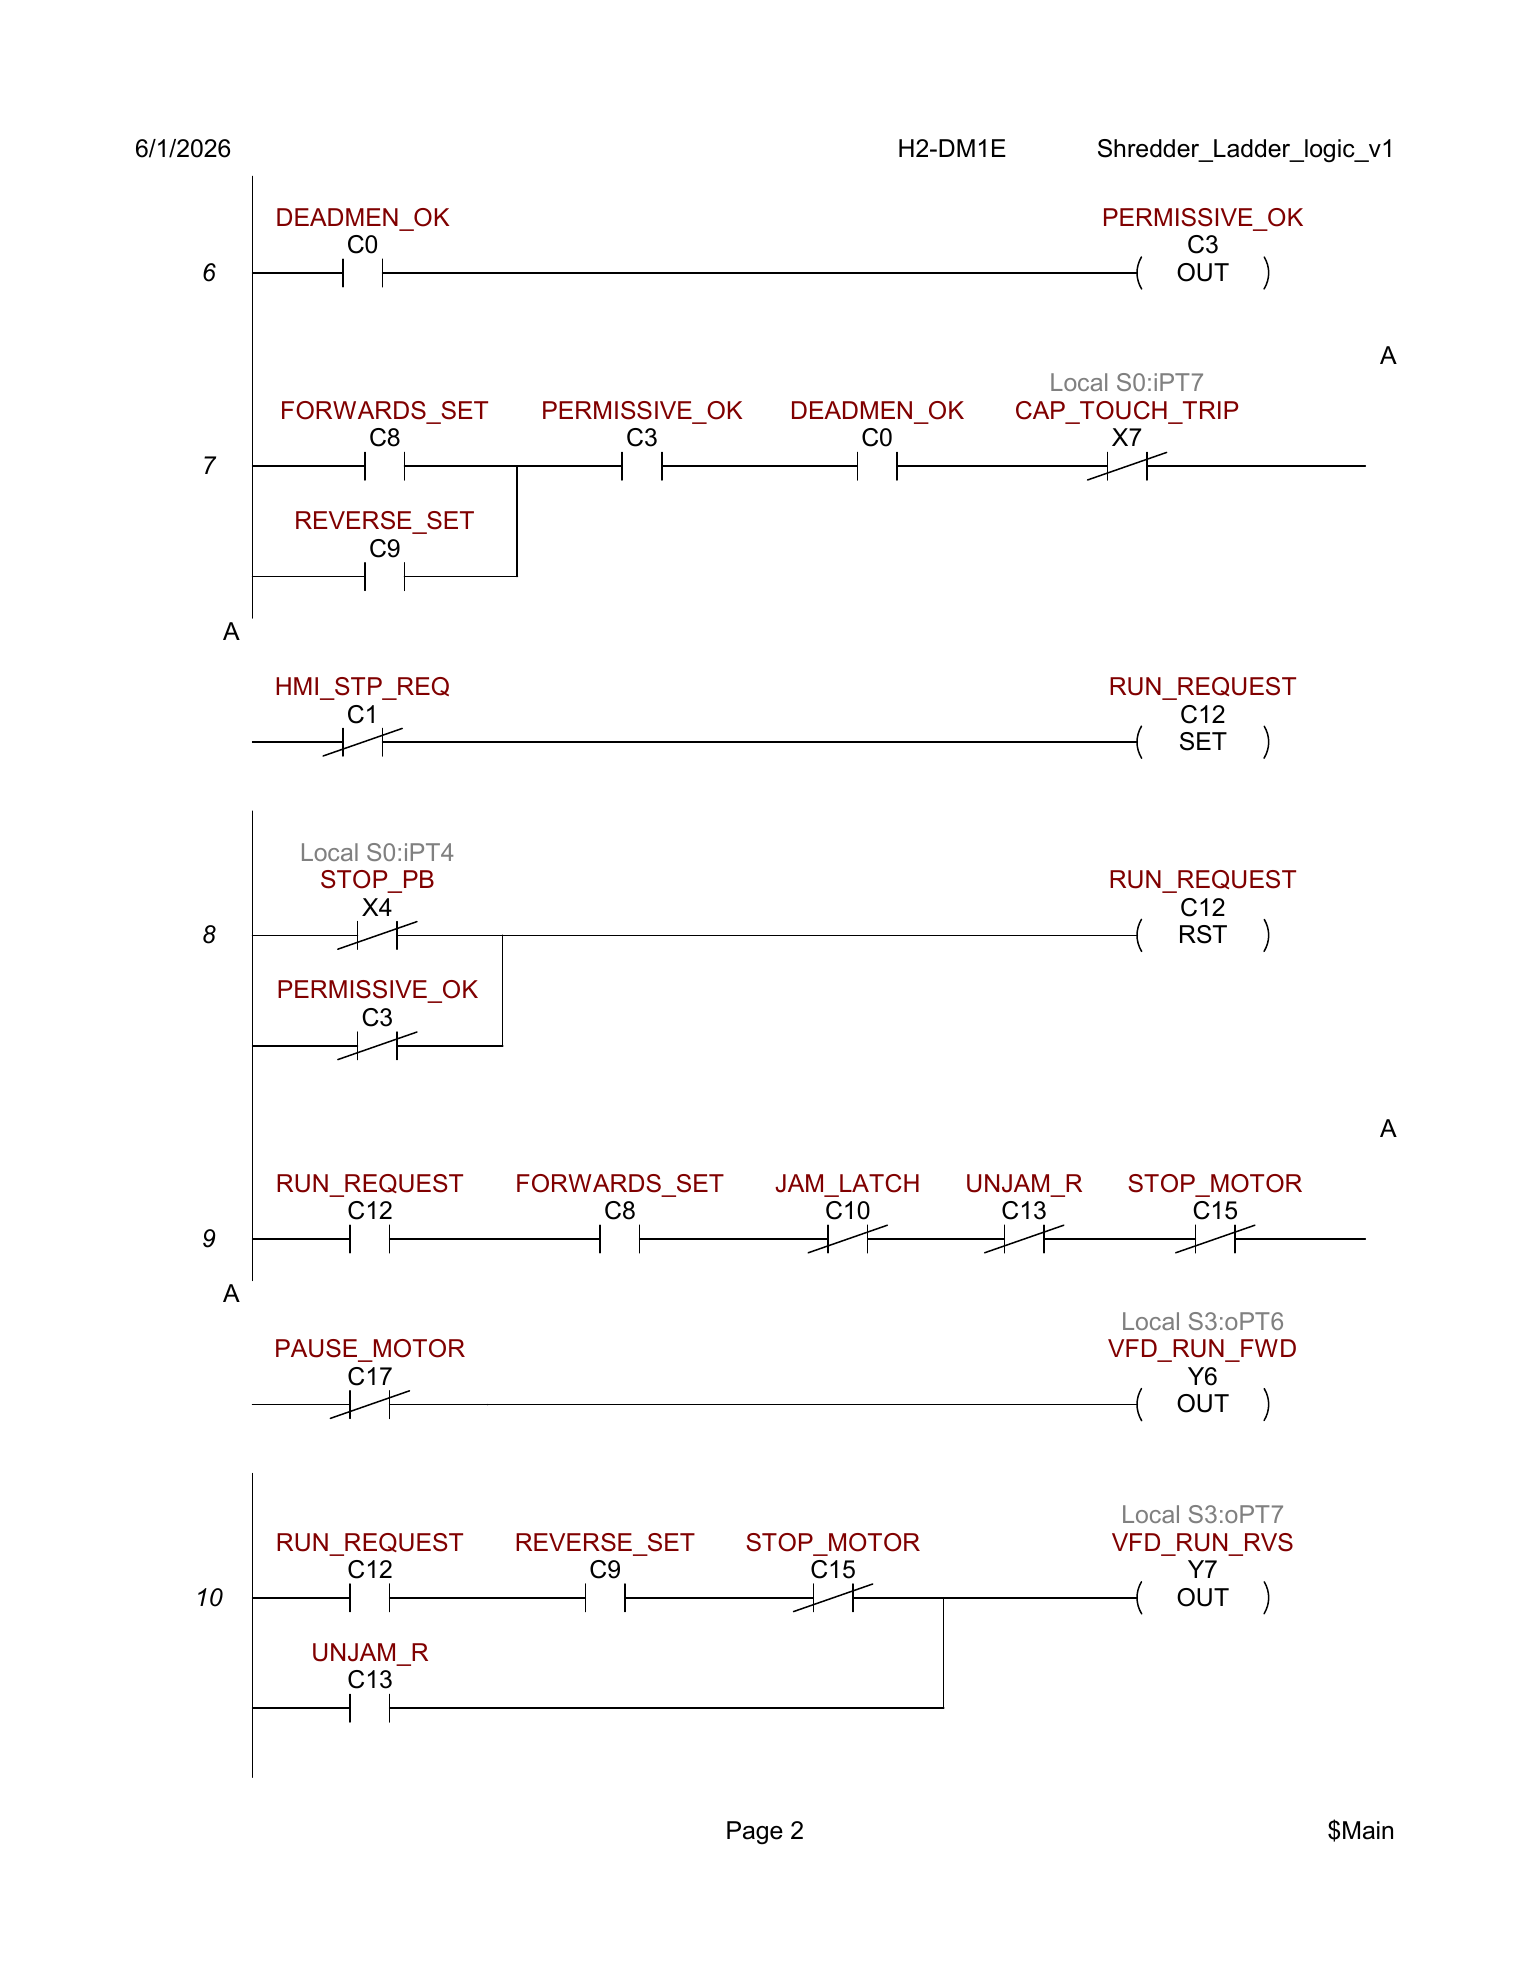
\includegraphics[height=2.1in]{./Pictures/Ladder_2.png}\\[6pt]
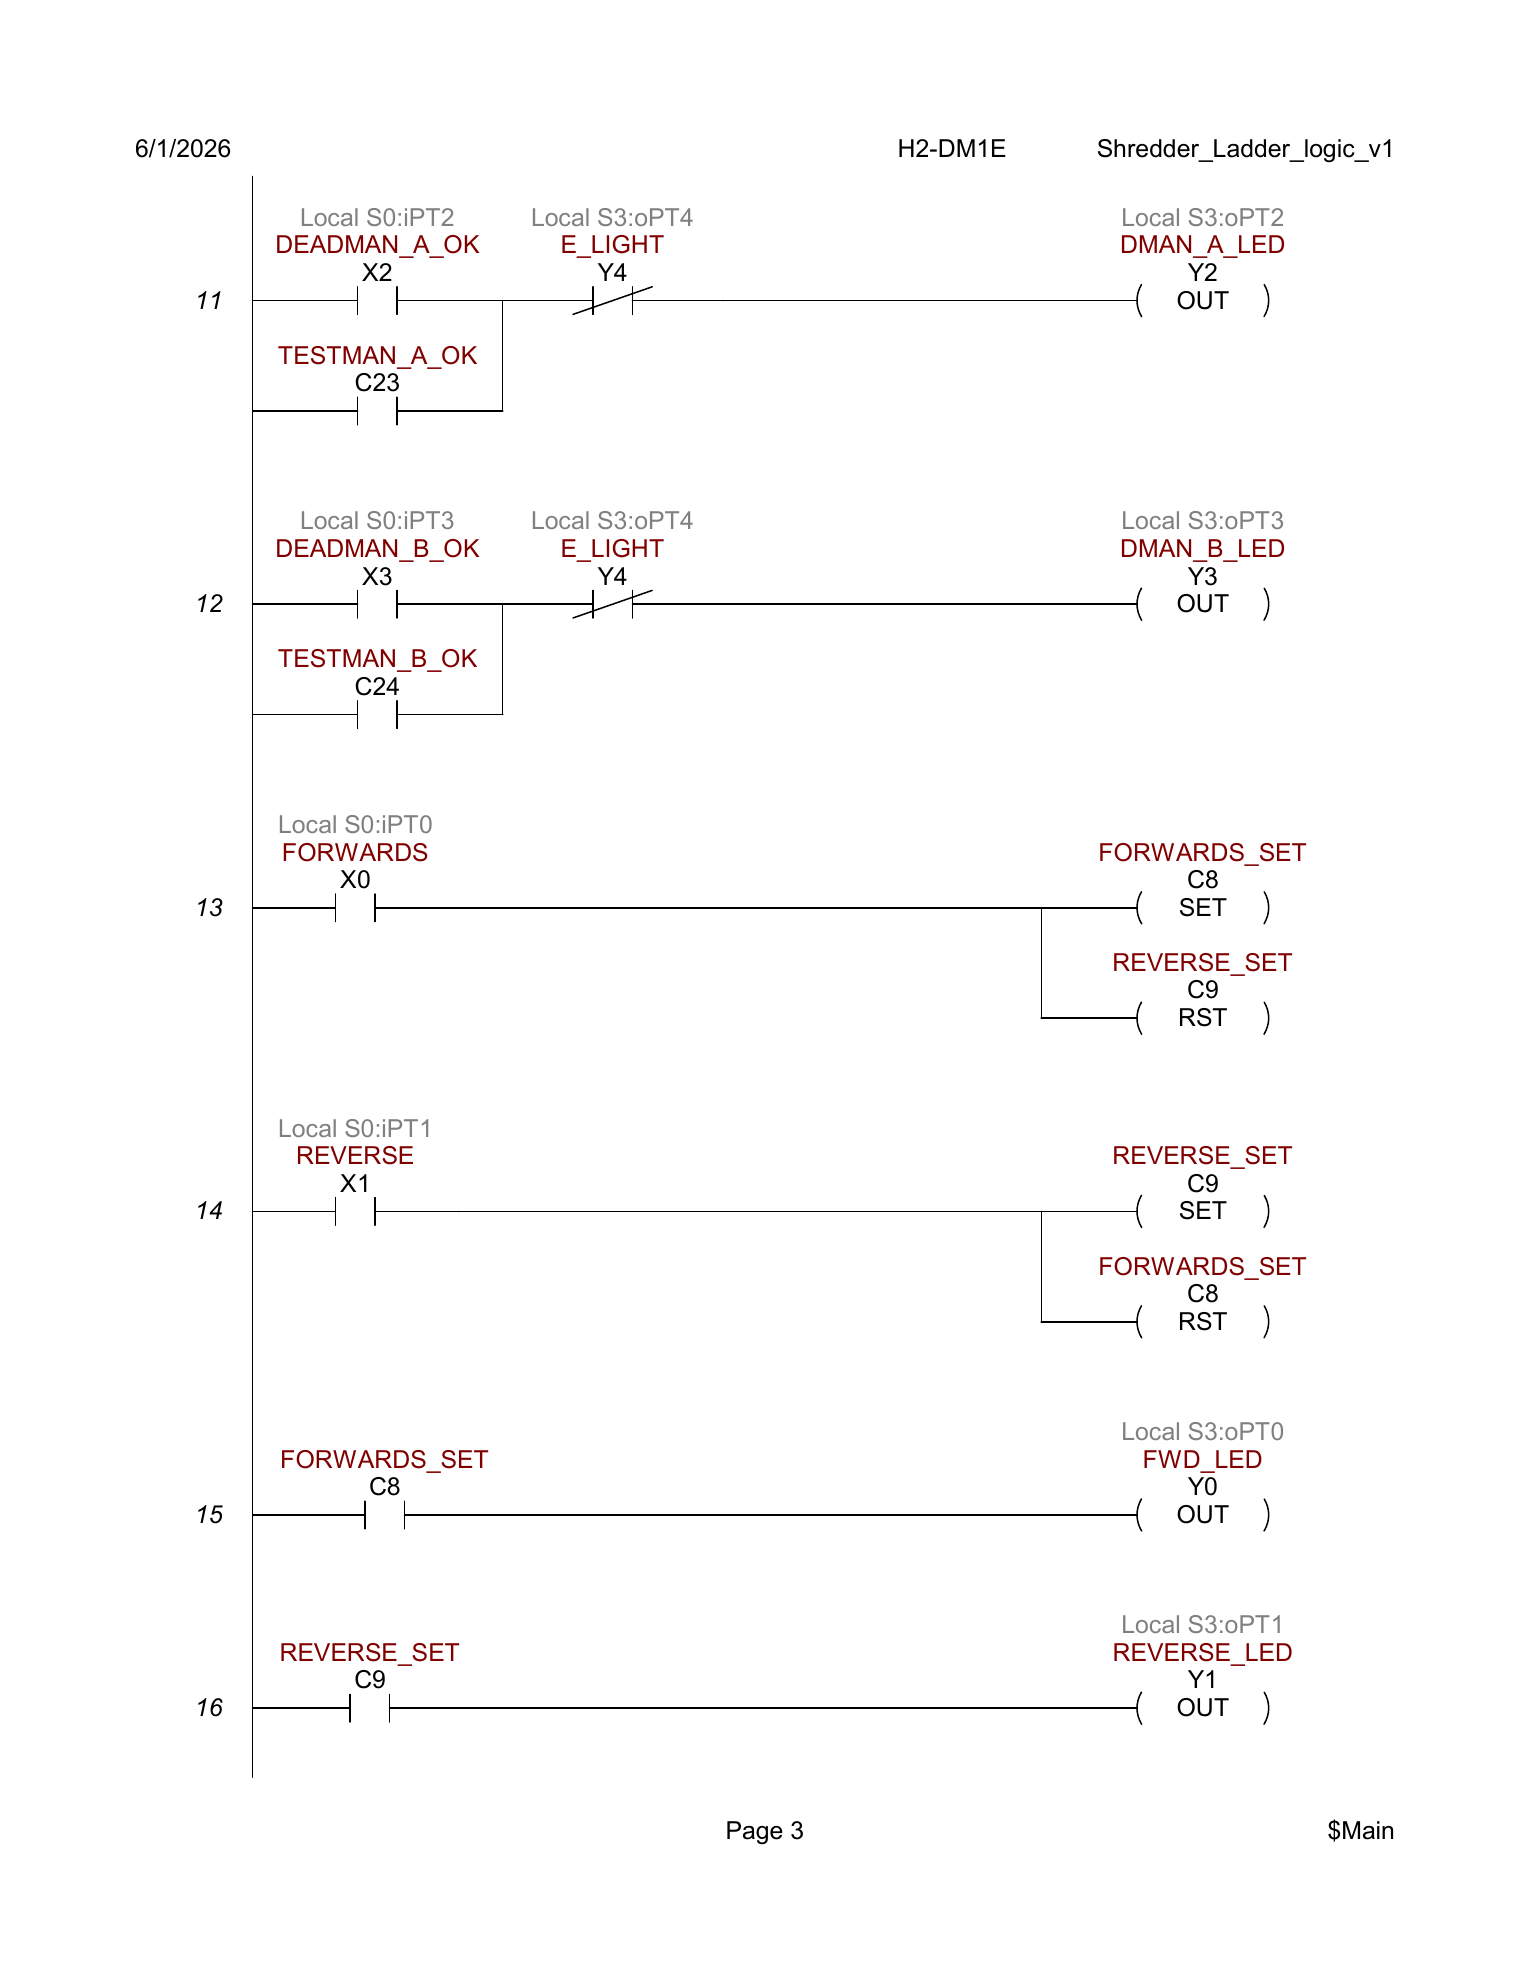
\includegraphics[height=2.1in]{./Pictures/Ladder_3.png}\hspace{6pt}%
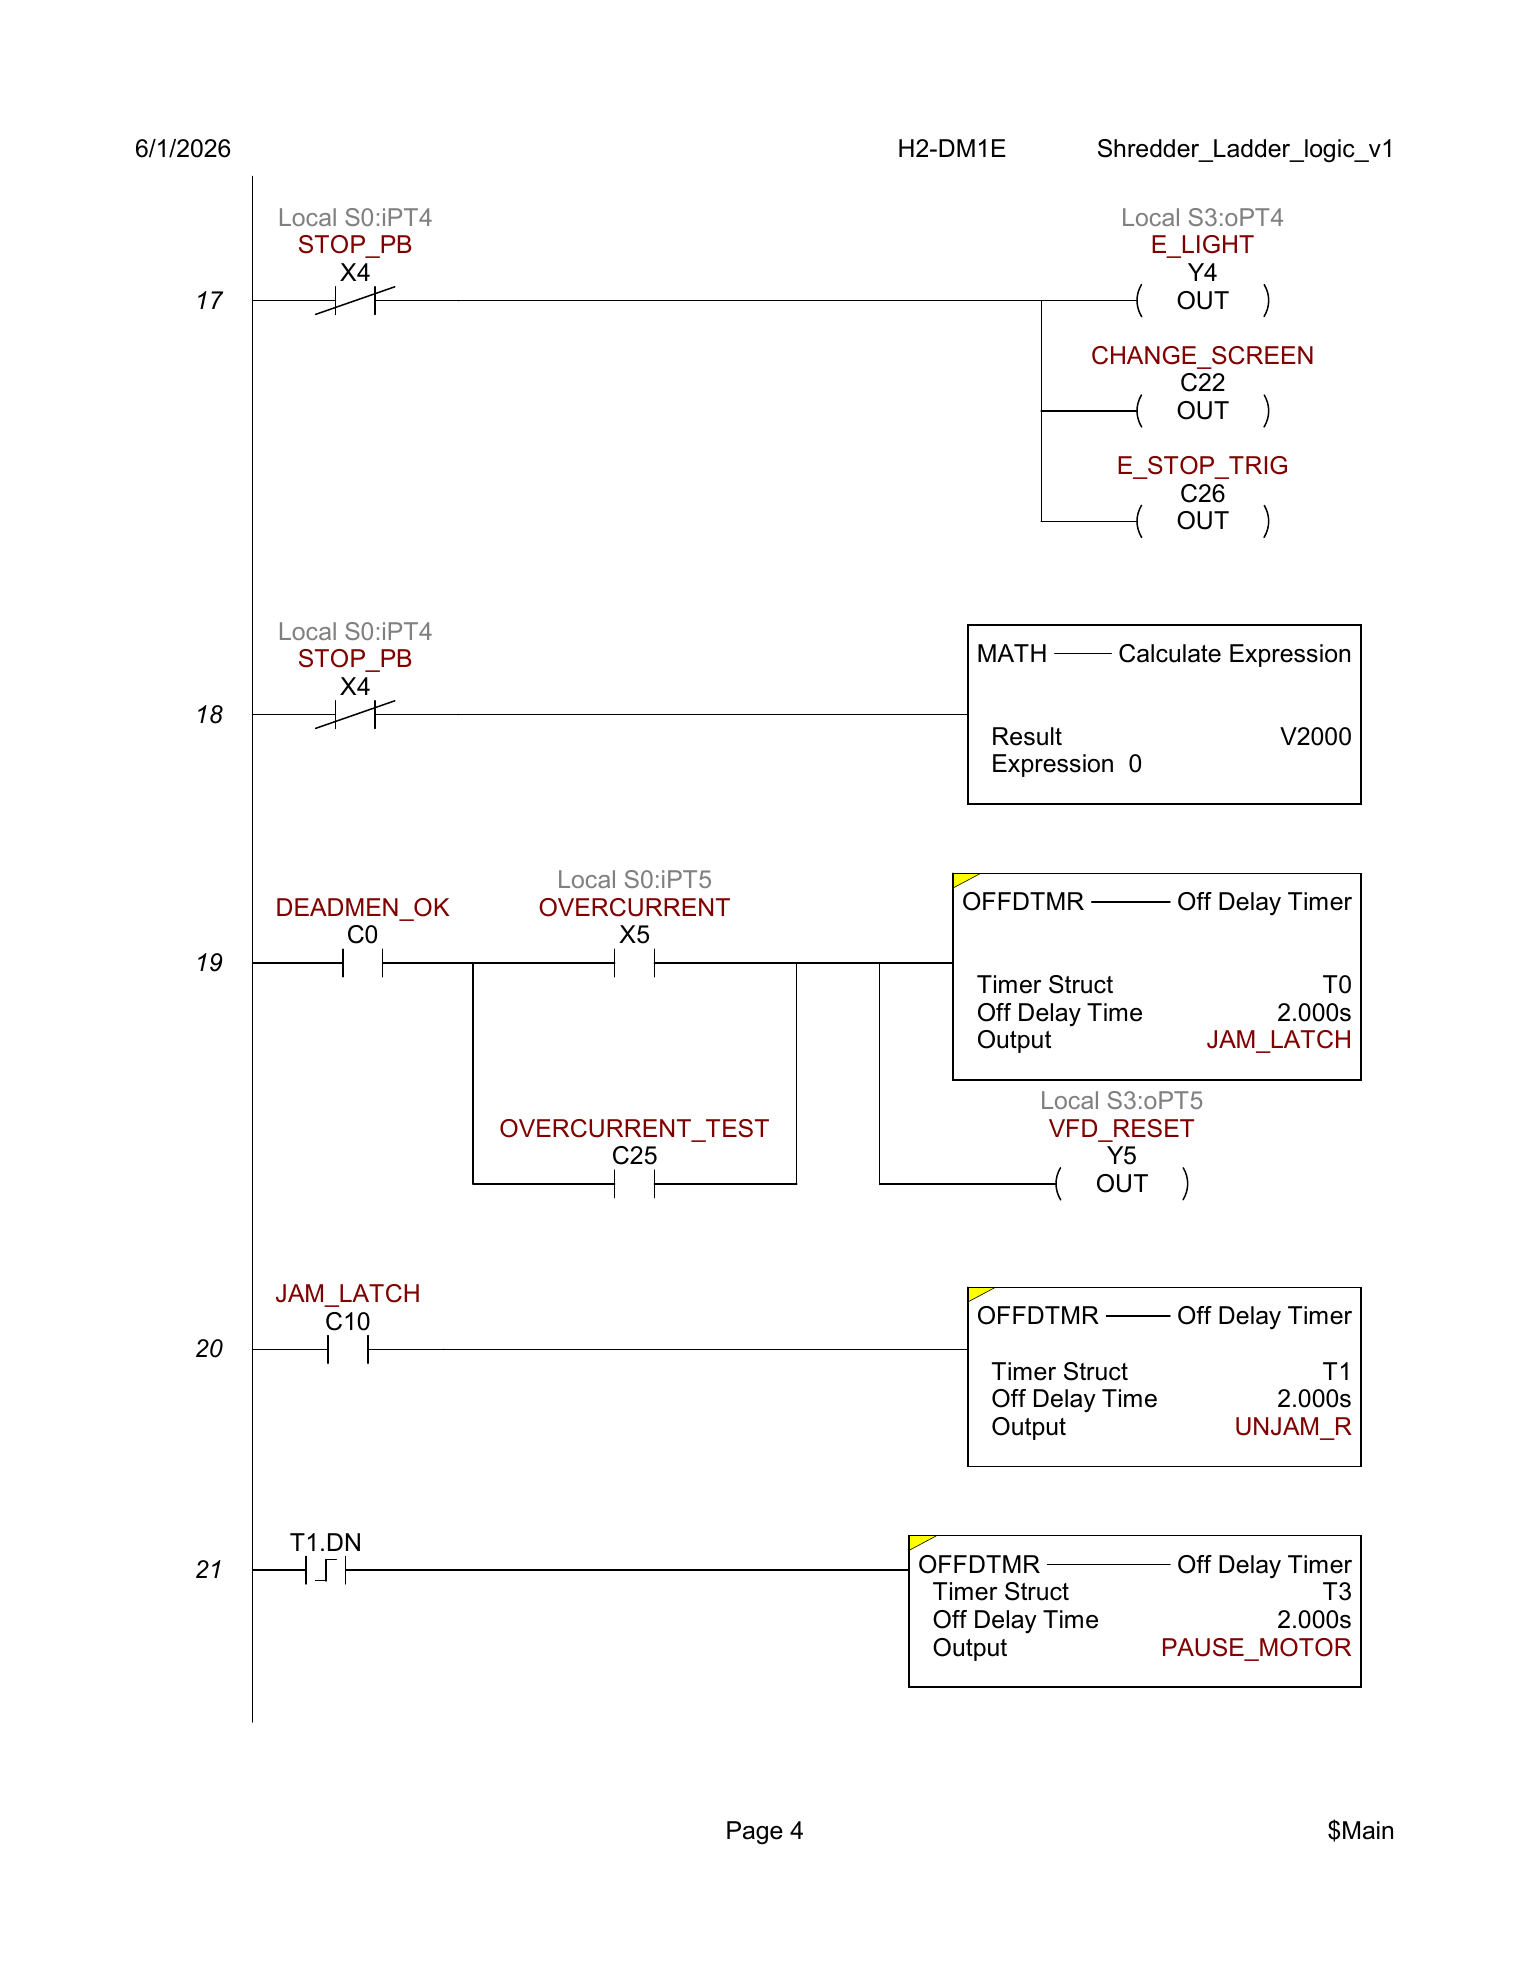
\includegraphics[height=2.1in]{./Pictures/Ladder_4.png}\\[6pt]
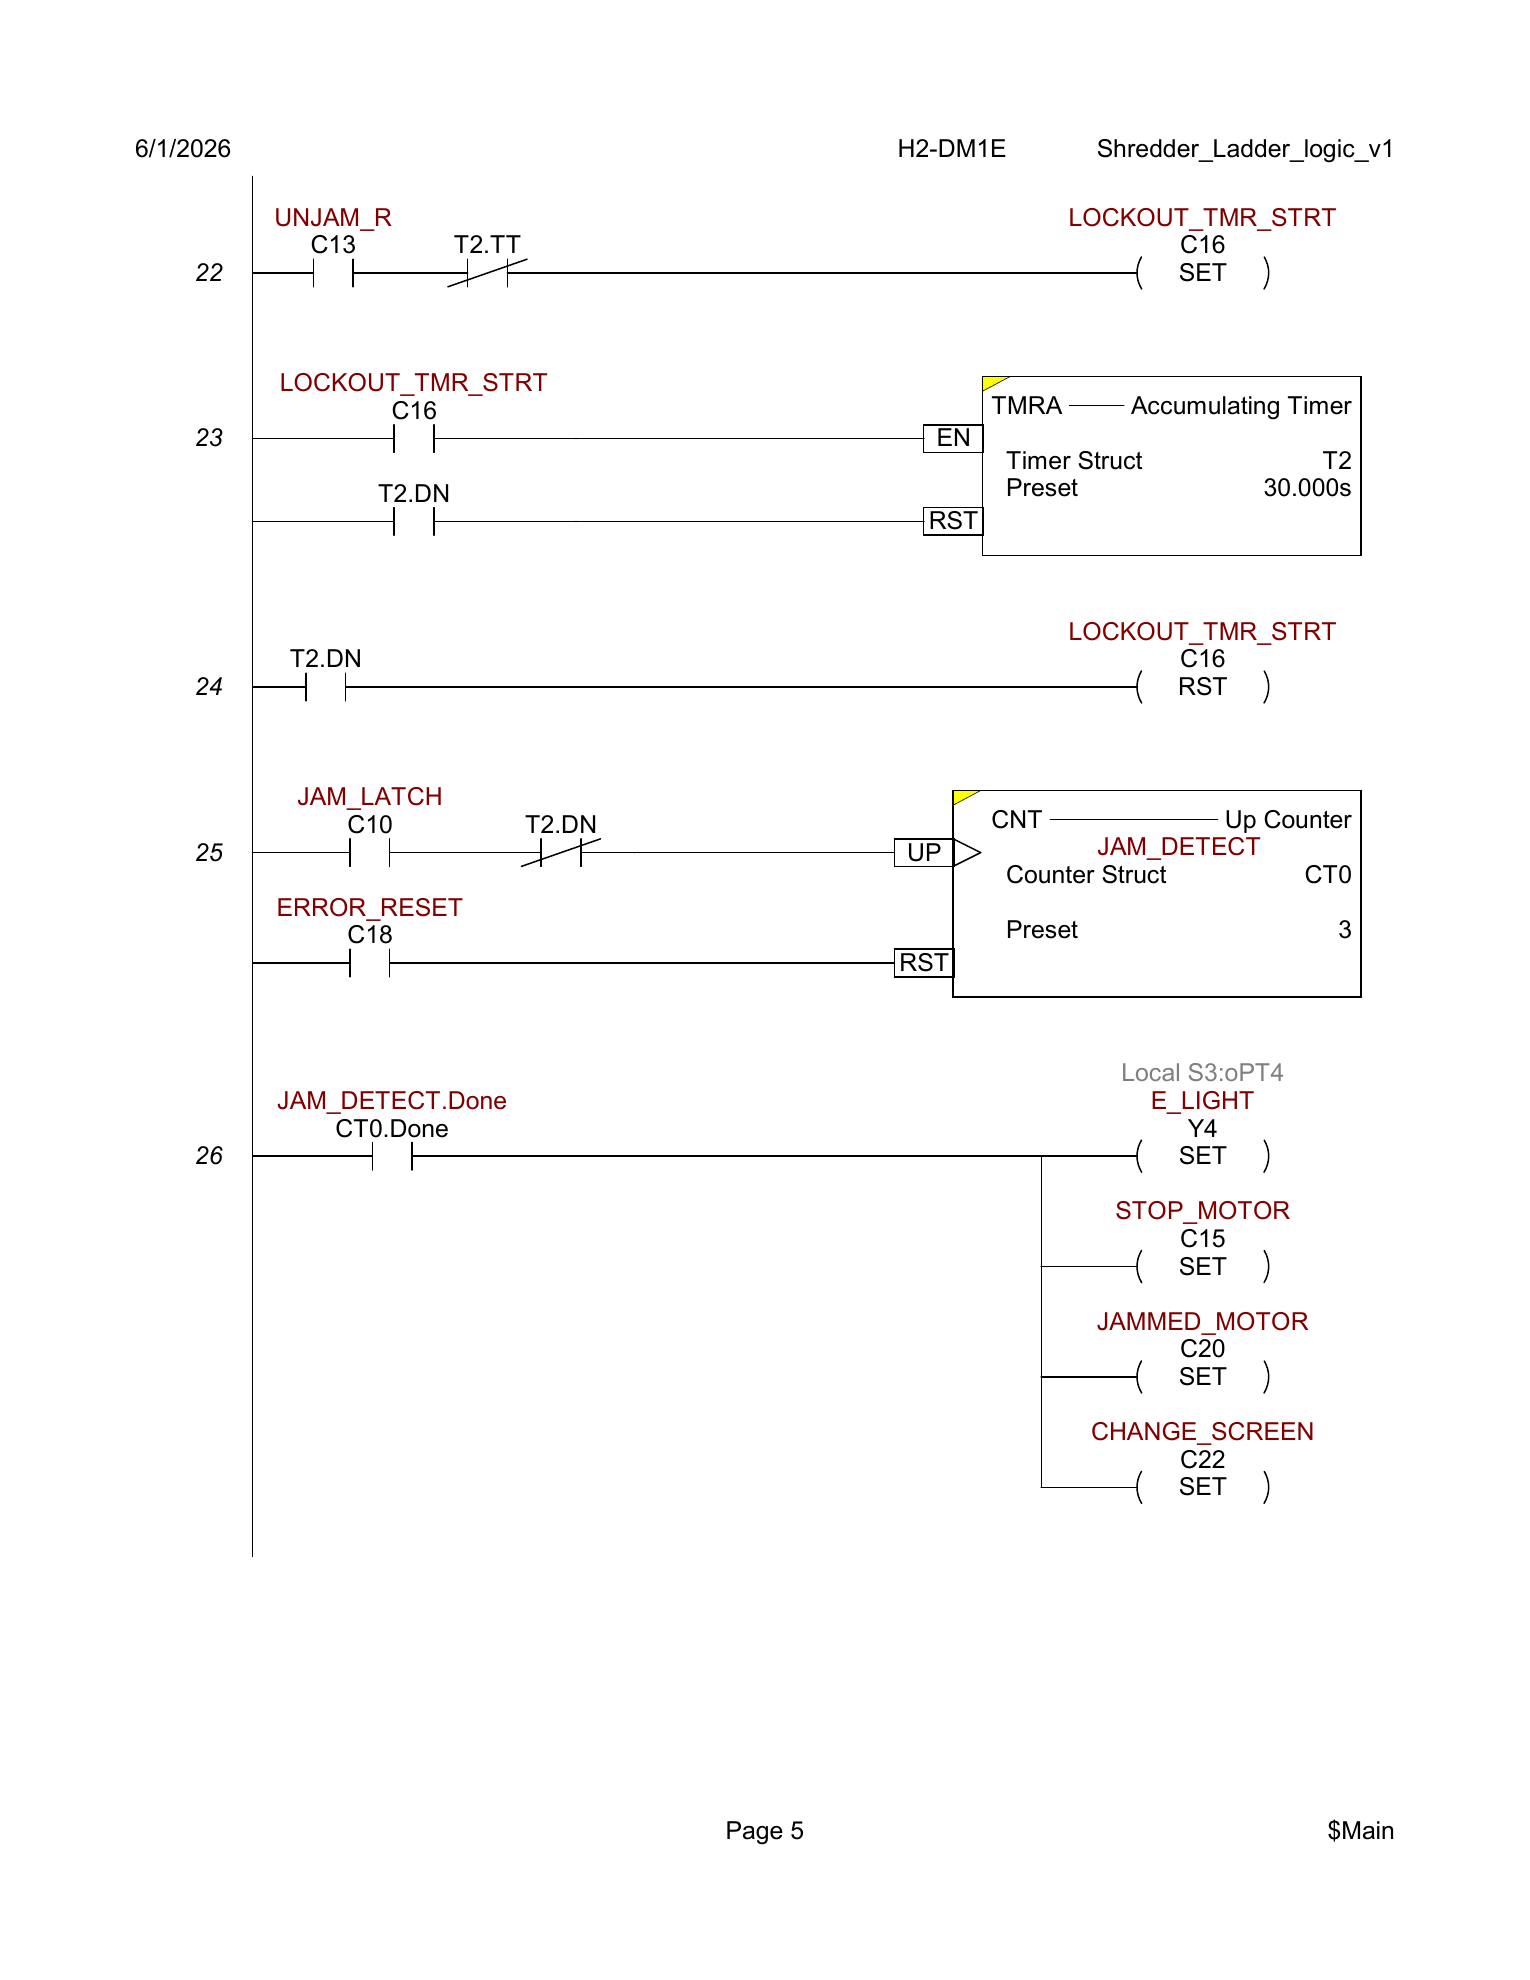
\includegraphics[height=2.1in]{./Pictures/Ladder_5.png}\hspace{6pt}%
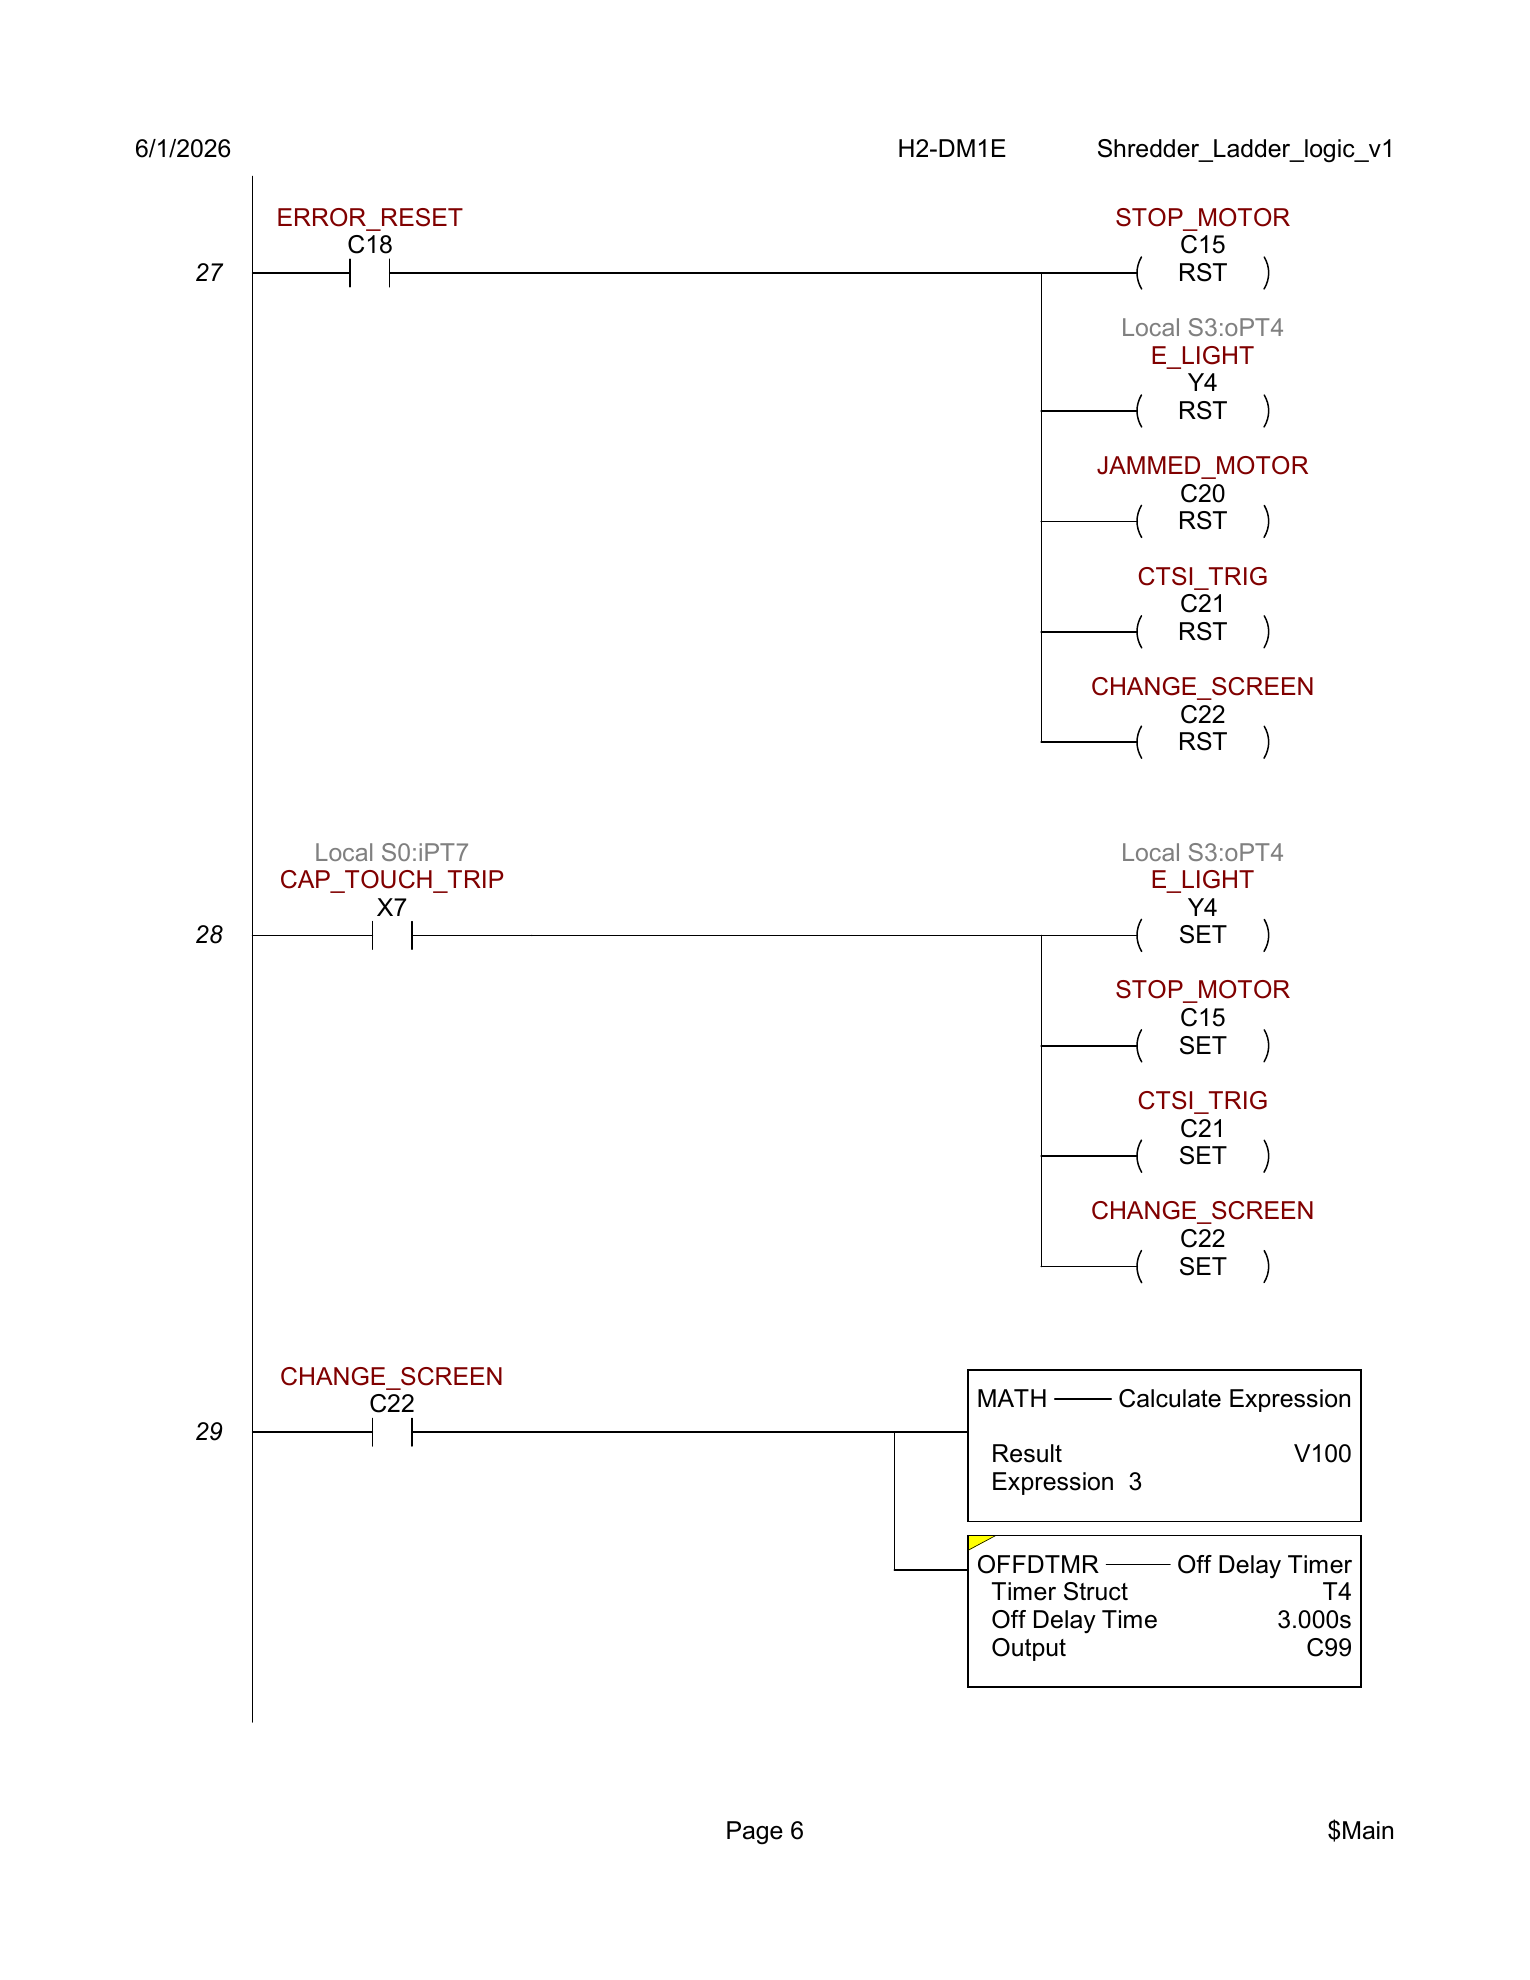
\includegraphics[height=2.1in]{./Pictures/Ladder_6.png}\\[6pt]
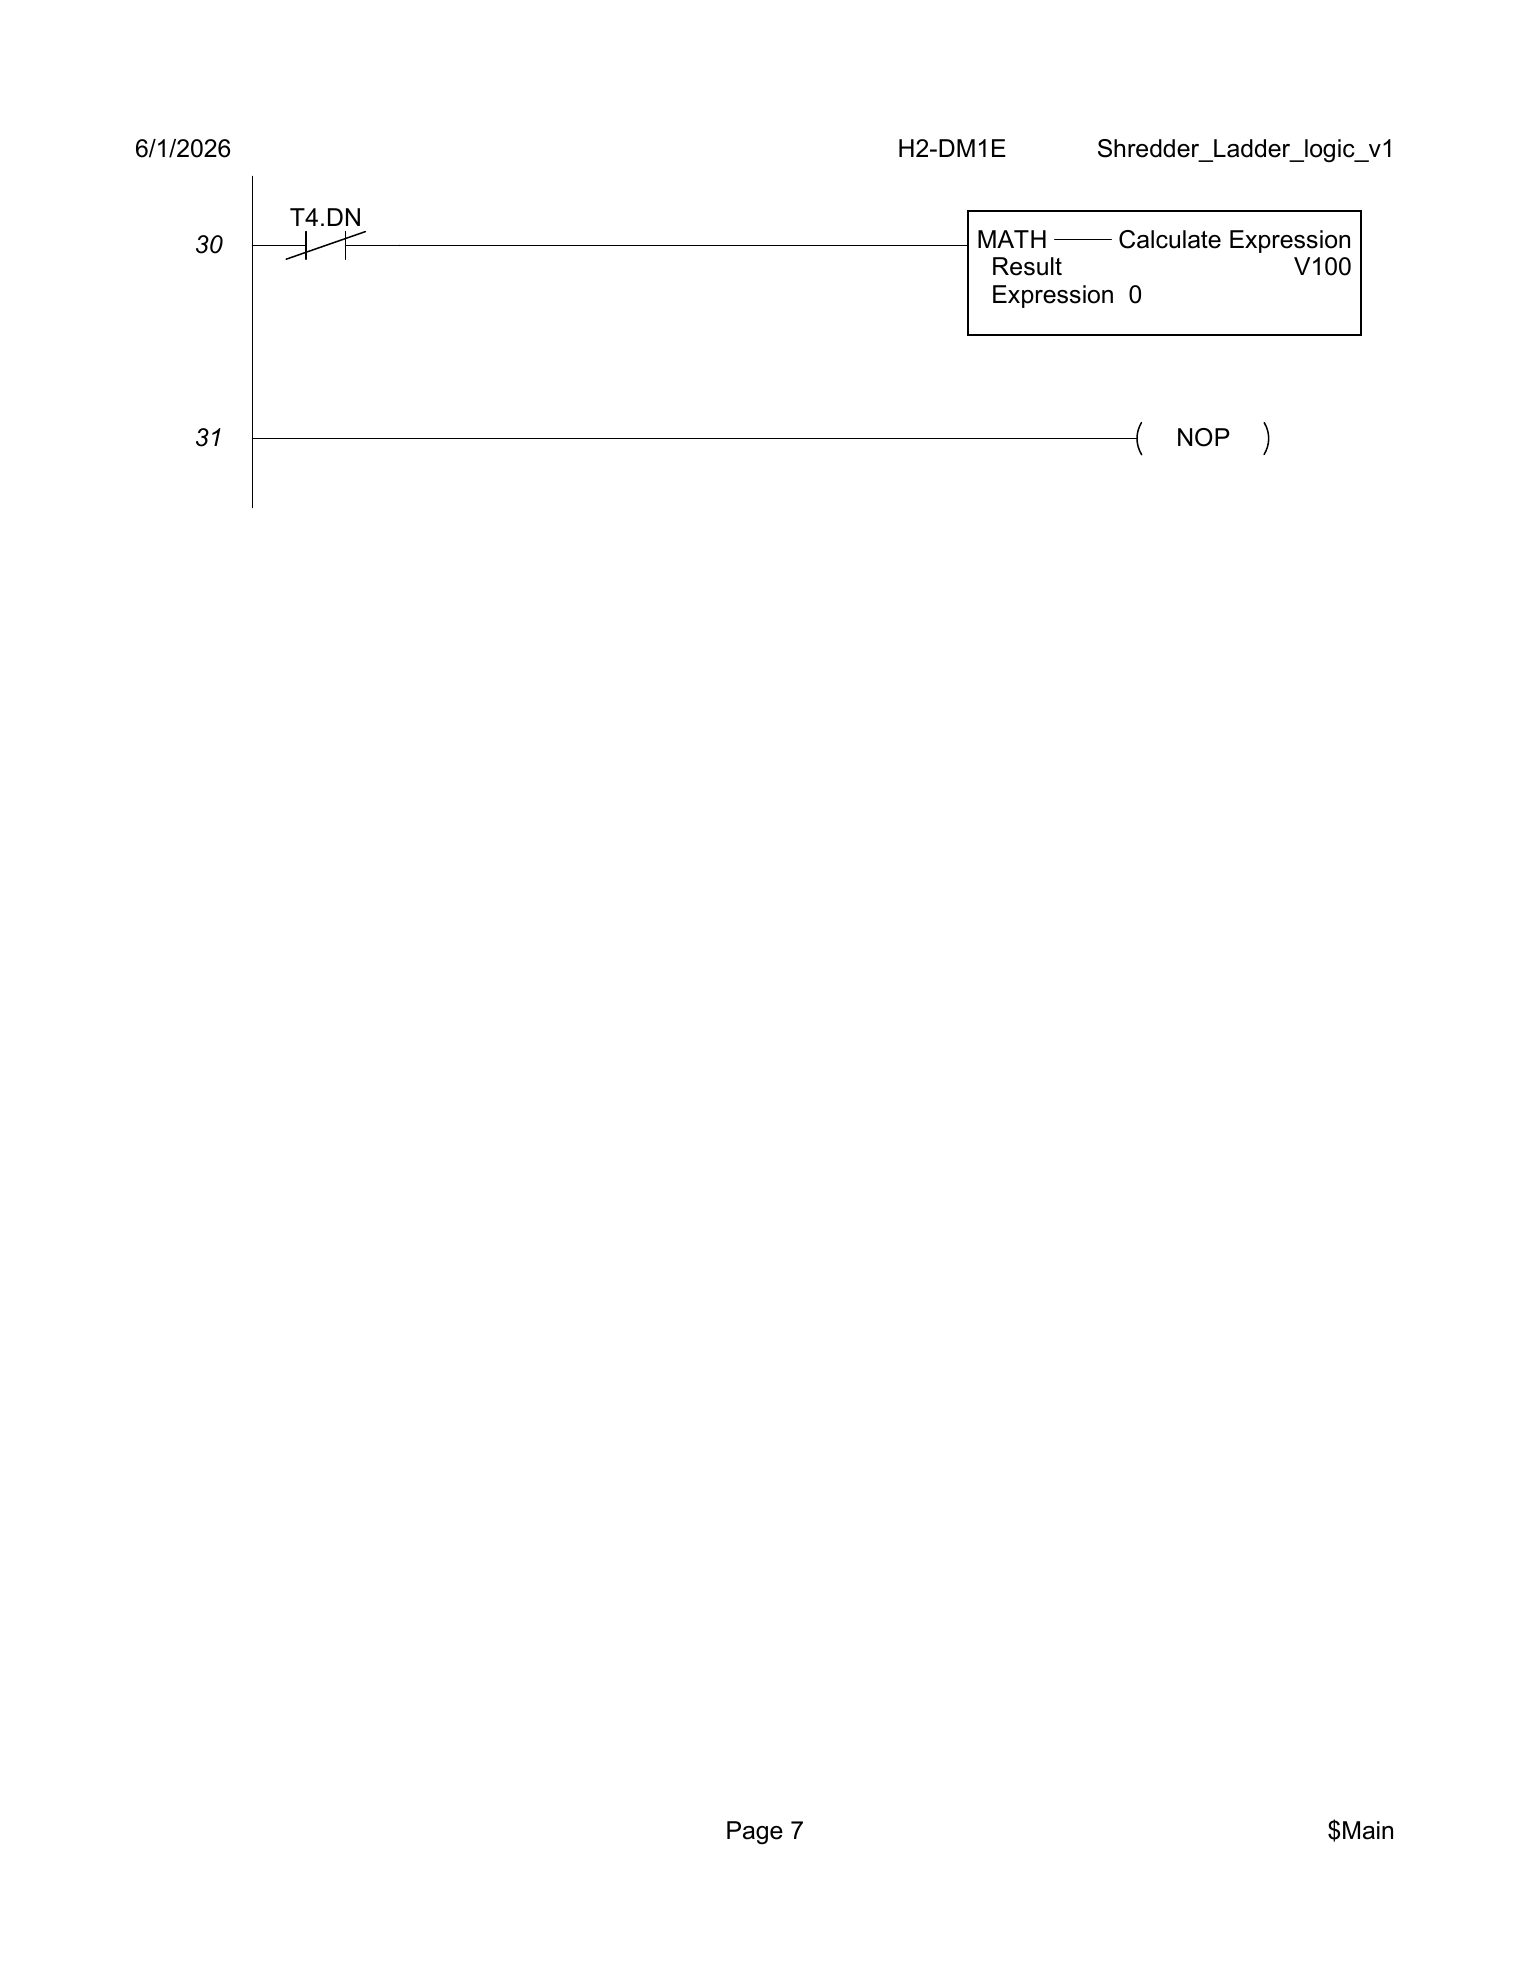
\includegraphics[height=2.1in]{./Pictures/Ladder_7.png}\\[2pt]
{\small\itshape All 31 ladder rungs (pages 1--7): init, deadman, RUN\_REQUEST gating, indicators, E-stop / jam detection, lockout, fault reset, screen change.}
\end{center}

\columnbreak
%================ COLUMN 3 ================
\postersec{HMI}
AutomationDirect EA1-T4CL C-more Micro-Graphic 4\,in.~touch panel
running \texttt{HMI\_413.mgp}, serial to the H2-DM1E CPU. Four
screens hold 27 PLC tags.

\begin{center}
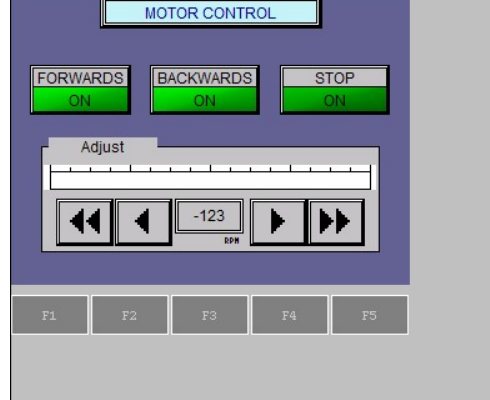
\includegraphics[width=0.48\columnwidth]{./Pictures/HMI_Motor_Control.png}\hspace{4pt}%
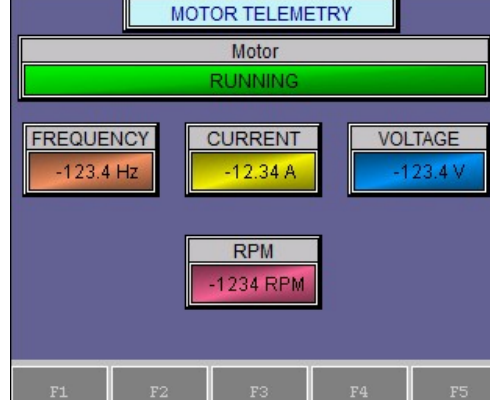
\includegraphics[width=0.48\columnwidth]{./Pictures/HMI_Telemetry.png}\\[3pt]
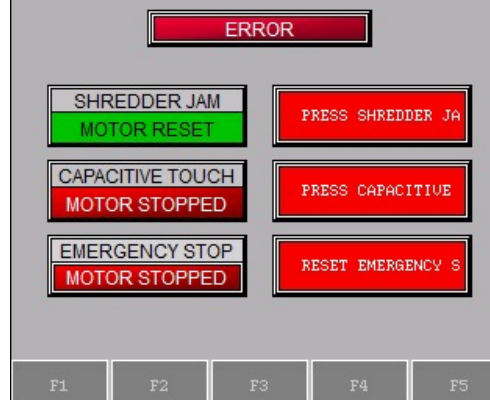
\includegraphics[width=0.48\columnwidth]{./Pictures/HMI_Error.png}\hspace{4pt}%
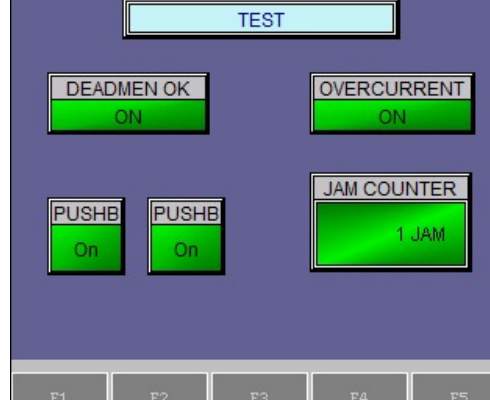
\includegraphics[width=0.48\columnwidth]{./Pictures/HMI_Test.png}\\[2pt]
{\small\itshape Motor Control, Motor Telemetry, Error / Alarm, Test.}
\end{center}

\postersec{Safety \& Compliance}
\begin{itemize}\setlength{\itemsep}{2pt}
  \item \textbf{E-stop:} Category 0 stop. Eaton E22B1 NC mushroom in series with the SD-N35 contactor coil. Drops the contactor independently of the PLC.
  \item \textbf{Two-hand / deadman:} both pushbuttons must be held to enable the motor (PLC X2 AND X3).
  \item \textbf{Overcurrent / jam:} VFD over-torque trip (\texttt{PD124 = 150\%}, \texttt{PD125 = 3\,s}) on PLC X5; ladder runs the 3-strike unjam routine.
  \item \textbf{Enclosure:} Vorksmen SEB001 steel, NEMA Type 12.
  \item \textbf{Compliance:} NFPA 70/79, NEMA 250 / ICS / MG~1, ISO 12100, 13849-1 (Cat~B--1 / PL b--c), 13850, 13851, OSHA 1910.147.
\end{itemize}

\postersec{Results}
\begin{itemize}\setlength{\itemsep}{2pt}
  \item Panel built, wired, bench-validated. All 31 rungs program and scan correctly.
  \item All four HMI screens operate; tag database matches the PLC.
  \item Speed reference verified: HMI \texttt{V2000} $\rightarrow$ \texttt{SCALE} $\rightarrow$ \texttt{F2-08DA-2 CH1} $\rightarrow$ VFD \texttt{VI}.
  \item Jam-recovery verified: overcurrent on \texttt{X5} $\rightarrow$ 2\,s reverse (\texttt{T1}) $\rightarrow$ coast-to-stop buffer (\texttt{T3}).
  \item Three-revision point list signed off by Fearghus Tyler.
\end{itemize}

\end{multicols}

% ============== BOTTOM FEATURE STRIP ==============
% Uses the white space below the multicol body.
\vspace{12pt}
\noindent
\begin{tcbraster}[raster columns=4, raster equal height, raster column skip=12pt,
  enhanced, sharp corners, boxrule=0pt, frame hidden,
  interior style={top color=PSUcream, bottom color=white},
  borderline north={4pt}{0pt}{PSUgreen},
  left=14pt, right=14pt, top=10pt, bottom=12pt,
  fonttitle=\sffamily\bfseries\large, coltitle=PSUgreen,
  attach title to upper={\par\smallskip},
  fontupper=\sffamily\normalsize,
]
\tcbitem[title=Project By the Numbers]
\textbf{31} ladder rungs in production. \\
\textbf{27} HMI tags across 4 screens. \\
\textbf{14} component sheets in the point list. \\
\textbf{3} strikes before the motor locks out. \\
\textbf{2 s} unjam reverse stroke. \\
\textbf{150\%} over-torque threshold on the VFD.

\tcbitem[title=Hardware Stack]
\textbf{PLC:} DirectLOGIC 205 + H2-DM1E. \\
\textbf{HMI:} C-more EA1-T4CL. \\
\textbf{VFD:} Huanyang HY02D211B-T. \\
\textbf{Motor:} GE 5KE182BC205B (3 HP bench). \\
\textbf{PSU:} Mean Well NDR-480-24. \\
\textbf{Contactor:} Mitsubishi SD-N35.

\tcbitem[title=Future Work]
Production motor selection (3--5\,HP) supersedes \texttt{PD141--PD144}. \\
Mechanical integration and shred-load run pending ME team. \\
Capacitive-touch (CTSI) module on \texttt{X7}: machine-level verification pending. \\
Optional Modbus link to the VFD for richer telemetry.

\tcbitem[title=Acknowledgments]
Thanks to \textbf{Bridget Lannigan} (MME / Ichor Systems) for sponsoring the project; to advisors \textbf{Prof.~Andrew Greenberg}, \textbf{Dr.~Jonathan Bird}, and \textbf{Robert Paxton}; and to the \textbf{PSU Power Engineering Laboratory} for bench access.\\[4pt]
\textit{ECE 412/413 Capstone Poster Session $\bullet$ PSU MCECS $\bullet$ June 12, 2026}
\end{tcbraster}

\end{document}
